\yboy{1}{
\ea\label{ex:argstr:intro:Tony:inf}
\gll Tony=nang naasi \textbf{ma}-maakang boole. \\
     Tony=\textsc{dat} cooked.rice \textsc{inf}-eat can  \\
    `Tony can eat rice.' (nosource)
\z
} \\
In \xref{ex:argstr:intro:Tony:inf}, we are deal

\chapter{Valency frames}\label{sec:argstr}
The different types of predicates discussed above can occur with different numbers of arguments which can be marked for various cases. In the following, we will deal with the valency structure \citep{Bickel2004syntexp}, or case frames \citep{Tsunoda2004issues}, of predicates taking between 1 and 3 arguments.\footnote{There seems to be no clear way to tell arguments from adjuncts in SLM, a property common to other Austronesian languages \citep[158]{Himmelmann2005typochar}.}

For predicates taking from one to three arguments, we will see whether its arguments are zero-marked, or whether the predicate assigns a particular case expressed by a certain postposition to its arguments. The postpositions of particular interest here are: \trs{=yang}{accusative}, \trs{=nang}{dative}, \trs{=dering}{instrumental}. The instrumental is somewhat peripheral as it can only be used with institutional actors like the police or the government. In this respect, it resembles English institutional plurals (\em The police are investigating\em) and Dutch feminine agreement for institutions (\trs{Het kabinet en haar beleid}{The cabinet[neuter] and her policy}). The use of \em =dering \em on core arguments is therefore limited to a small semantic class of entities and does not form part of SLM core grammar, so that its importance for the SLM alignment system should not be overestimated. Another issue is the dative marking found in predicates with a modal preclitic on the verb. For instance, we get zero marking in \xref{ex:argstr:intro:Tony:zero}, but dative marking in \xref{ex:argstr:intro:Tony:dat}, where the modal preclitic \em bole= \em is present.


\yboy{2}{
\ea \label{ex:argstr:intro:Tony:zero}
\gll Tony naasi arà-maakang. \\
     Tony cooked.rice \textsc{non.past}-eat  \\
    `Tony eats rice.' (nosource)
\z
} 
\yboy{2}{
\ea \label{ex:argstr:intro:Tony:dat}
\gll  Tony=\textbf{nang} naasi \textbf{bole=}maakang. \\
      Tony=\textsc{dat} cooked.rice can=eat \\
    `Tony can eat rice.' (nosource)
\z
} \\
The dative case on \em Tony \em is thus not assigned by the verb \trs{maakang}{eat}, but by the preclitic \trs{bole=}{can}. Given the tight integration of the preclitic with its host, it is difficult to argue that we are dealing with two clauses here. Such a biclausal analysis is possible for the alternative form with a free word \em boole \em and the infinitive \em mà- \em given in \xref{ex:argstr:intro:Tony:inf}.


\yboy{1}{
\ea\label{ex:argstr:intro:Tony:inf}
\gll Tony=nang naasi \textbf{ma}-maakang boole. \\
     Tony=\textsc{dat} cooked.rice \textsc{inf}-eat can  \\
    `Tony can eat rice.' (nosource)
\z
} \\
In \xref{ex:argstr:intro:Tony:inf}, we are dealing with a modal predicate \em boole\em, which assigns dative to \em Tony \em and infinitive to \em maakang\em. In the former case with the preclitic \em bole=maakang\em, such a biclausal analysis is problematic. When \em bole= \em is used, arguments of every predicate type can take dative marking. We will list these predicates, but as with \em =dering\em, the importance of dative assigned by modal preclitics should not be overestimated when determining the SLM alignment system.



\section{One-place predicates}\label{sec:argstr:One-placepredicates}
One-place predicates are predicates with only one argument. Very often, the argument does not carry any case marking because the relation between it and the predicate is clear and there is no need for disambiguation, another argument not being present.  The following two examples show the lack of marking for an actor \xref{ex:pred:argstr:1:zero:actor} and an undergoer \xref{ex:pred:argstr:1:zero:undergoer}.
 
\yboy{1}{
\ea\label{ex:pred:argstr:1:zero:actor}
\gll itthukapang      Tony Hassan=\zero{} su-pii. \\ % bf
      then Tony Hassan \textsc{past}-go \\
    `Then Tony Hassan left.' (K060116nar09)
\z
} \\
\yboy{1}{
\ea\label{ex:pred:argstr:1:zero:undergoer}
\gll dee=\zero{} su-thiidor     baawa=ka. \\ % bf
     \textsc{3s} \textsc{past}-sleep down=\textsc{loc}  \\
\z
} \\
Psychological and physiological predicates can assign the dative, as in \xref{ex:pred:argstr:1:dative}, where the predicate \trs{thàràsiggar}{sick} assigns dative case to the experiencer of the sickness, \em go\em, yielding \em godang \em \citep[cf.][]{Ansaldo2005ms,Ansaldo2008genesis, Ansaldo2009}. The marking of this type of predicates with the dative is typical for South Asia \citep[159ff]{Masica1976}.
 
\yboy{1}{
\ea\label{ex:pred:argstr:1:dative}
\gll go\textbf{dang}    karang bannyak thàràsiggar. \\
     1s.familiar=dat now very sick  \\
    `I am now very sick.' (B060115nar04)
\z
} \\
Institutions take the instrumental \em =dering\em, also on one-place predicates.\footnote{See \citet[791]{Gair2003} for institutional actors being marked with the instrumental in Sinhala.}

\yboy{1}{
\ea
\gll {\em police}=\textbf{dering} su-dhaathang. \\
     police=instr \textsc{past}-come  \\
    `The police came.' (nosource)
\z
} \\
When dealing with modal predicates, one place predicates can also mark dative on their argument. This is shown in \xref{ex:pred:argstr:1:dative:modal}. Normally, \trs{duuduk}{stay} would not assign dative case to its argument, but when prefixed with \em bole= \em it does.

\yboy{1}{
\ea\label{ex:pred:argstr:1:dative:modal}
\gll   kithang=\textbf{nang}   \el{}    2 {\em o'clock}=ke=sangke  bole=duuduk. \\
      \textsc{1pl}=\textsc{dat} { }    two o'clock=\textsc{simil}=until can-stay  \\
    `We can stay up until 2 o' clock.' (K061026rcp04)
\z
} \\
In some instances, the accusative marker \em =yang \em can be found as the argument of a one-place predicate.\footnote{\citet[791]{Gair2003} states for Sinhala that `accusative subjects' imply lack of volition and ``that some external force is responsible,'' which is indeed the case for the Titanic in example \xref{ex:pred:argstr:1:dative:modal}.}



\yboy{1}{
\ea\label{ex:pred:argstr:1:acc:titanic}
\gll {\em Titanic} kappal=\textsc{yang} su-thìnggalam. \\
     Titanic ship=\textsc{acc} \textsc{past}-sink  \\
\z
} \\
In those cases, care must be taken to check whether we are dealing with a true one-place predicate, or with a two-place predicate where the actor argument is dropped. For instance, the verb \em braanak \em is used to refer to child birth, and sentences like \xref{ex:pred:argstr:1:acc:braanak:intr} can be found, where there is only one argument, which is marked with \em =yang\em.



\yboy{1}{
\ea\label{ex:pred:argstr:1:acc:braanak:intr}
\gll   Itthu=subbath=jo      incayang=\textbf{yang}    siithu anà-braanak. \\
  therefore=\textsc{foc} \textsc{3s.polite}=\textsc{acc} there \textsc{past}-braanak   \\
\z
} \\
However, the verb \em braanak \em is a two-place predicate meaning `to give birth', as in clear from \xref{ex:pred:argstr:1:acc:braanak:tr} where both arguments are realized. In \xref{ex:pred:argstr:1:acc:braanak:intr}, and most other cases, the mother is not mentioned, giving the impression that \em braanak \em takes only one argument.

\yboy{1}{
\ea\label{ex:pred:argstr:1:acc:braanak:tr}
\gll umma seeyang su braanak. \\
     mother \textsc{1s}=\textsc{acc} past give.birth  \\
    `My mother gave birth to me.' (nosource)
\z
} \\
To return to example \xref{ex:pred:argstr:1:acc:titanic} about the Titanic, is is fortunately possible to show that the verb \trs{thìnggalam}{sink} is intransitive because it is one of the rare verbs where the transitive form is suppletive, \em cullop\em. If an actor causes the sinking of an undergoer, \em thìnggalam \em cannot be used, but \em cullop \em must be used instead. This entails that the sentence \em Titanic=yang su-thìnggalam \em has indeed accusative marking on the only argument of the predicate.
% 
% \yboy{1}{
% \ea
% \gll see *yang su laaher. \\
%        \\
%     `.' (nosource)
% \z
% } \\
% 
% 
% 
% 
% \yboy{1}{
% \ea
% \gll umma seeyang su kìnna braanak. \\
%        \\
%     `I was born accidentally (by my mother).' (nosource)
% \z
% } \\

Another instance where we find accusative marking on one-place predicates are existentials. This is not very frequent, and the exact circumstances for this are unclear. Specificity of the theme seems to favour the occurrence of \em =yang\em.\footnote{Specificity is also seen as an important factor in \citet{Ansaldo2005ms}, but only as far as the occurence of \em =yang \em on `objects' is concerned. The examples given below would probably not qualify as `objects', but specificity still plays a role in the occurence of \em =yang\em.} In example \xref{ex:pred:argstr:1:acc:assert} \em =yang \em is optional, but the informants feel that the sentence is better with \em =yang \em. Note that the hat is definite in \xref{ex:pred:argstr:1:acc:assert}, indicated by the deictic \em itthu\em.
\yboy{1}{
\ea\label{ex:pred:argstr:1:acc:assert}
\gll itthu thoppi=(yang) siini aada. \\
     \textsc{dist} hat=\textsc{acc} here exist  \\
    `That hat is here.' (nosource)6.11.08 better with yang
\z
} \\


Another instance where we find \em =yang \em is with some adjectival predicates \xref{ex:pred:argstr:1:acc:adj:seelon}\xref{ex:pred:argstr:1:acc:adj:bag}. As of now, there is no good explanation for these cases.


\yboy{1}{
\ea\label{ex:pred:argstr:1:acc:adj:seelon}
\gll Seelon=pe duppang muusing=yang bannyak panthas anthi aada. \\
     Sri Lanka=\textsc{poss} future time=\textsc{acc} much beautfiul \textsc{irr}-exist  \\
    `Sri Lanka's future will be bright.' (nosource)3.11.08
\z
} \\

\yboy{1}{
\ea\label{ex:pred:argstr:1:acc:adj:bag}
\gll itthu {\em bag}=yang lorang=nang bannyak bìrrath (\textbf{liiwath}). \\
     \textsc{dist} bag=\textsc{acc} \textsc{2pl}=\textsc{dat} much heavy more  \\
\z
} \\

When questioning the location of a specific referent, \em =yang \em is obligatory, as shown in \xref{ex:pred:argstr:1:acc:interr}.

\yboy{1}{
\ea\label{ex:pred:argstr:1:acc:interr}
\gll itthu thoppi=*(yang) aapaka aada. \\
     \textsc{dist} hat=\textsc{acc} what=inside exist  \\
    `Inside of what is that hat located?' (nosource)6.11.08
\z
} \\
A naturalistic example of \em =yang \em occuring on the argument of a locational predicate is \xref{ex:pred:argstr:1:acc:naturalistic}.


\yboy{1}{
\ea\label{ex:pred:argstr:1:acc:naturalistic}
\gll  3  {\em miles} cara  jaau=ka    aada  [dee anà-sbuuni   duuduk     {\em cave}]=yang. \\
      3 miles way far=\textsc{loc} exist \textsc{3s.familiar} \textsc{past}-hide stay cave=\textsc{acc} \\
\z
} \\
To sum up, arguments of monovalent predicates can be marked with zero or the dative. In exceptional cases, they can also be marked with the instrumental or the accusative. If modal preclitics are considered, the proportion of dative marking increases.




\section{Two-place predicates}\label{sec:argstr:Two-placepredicates}
With two place predicates, we have to distinguish the actor argument and the undergoer argument. Case marking of these arguments is optional.
\xref{ex:pred:argstr:2:zero:maakang} and \xref{ex:pred:argstr:2:zero:poothong} give sentences where both   arguments lack a postposition.

\yboy{1}{
\ea \label{ex:pred:argstr:2:zero:maakang}
\gll  Sebastian=\zero{} saathe=\zero{} asamaakang   aada=si. \\ % bf
     Sebastian satay \textsc{cp}-eat exist=\textsc{interr} \\
\z
} \\ 
\yboy{1}{
\ea \label{ex:pred:argstr:2:zero:poothong}
\gll  baapa=\zero{}  \el  hatthu pohong=\zero{} nya-poothong. \\ % bf
      father \textsc{3pl}=\textsc{poss} garden=\textsc{loc} \textsc{indef} tree \textsc{past}-cut \\
\z
} \\
While \trs{poothong}{cut} above was construed with two non-marked arguments, it is also possible to use the accusative on the undergoer, as shown in \xref{ex:pred:argstr:2:zeroacc}.


\yboy{1}{
\ea \label{ex:pred:argstr:2:zeroacc}
\gll  ithukapang       lorang=pe     leher=\textbf{yang}   kithang=\zero{} athi-poothong. \\
      then \textsc{2pl}=\textsc{poss} neck=\textsc{acc} \textsc{1pl} \textsc{irr}-cut \\
\z
} \\
Some verbs assign dative case to the undergoer argument, such as \trs{banthu}{help} in \xref{ex:pred:argstr:2:zerodat:banthu} or  \trs{puukul}{hit} in \xref{ex:pred:argstr:2:zerodat:puukul}.
 

\yboy{1}{
\ea\label{ex:pred:argstr:2:zerodat:banthu}
\gll derang pada=\zero{} arà-banthu cinggala  raaja=\textbf{nang}. \\
     \textsc{3pl} \textsc{pl} \textsc{non.past}-help Sinhala king=\textsc{dat}  \\
\z
} \\
\yboy{1}{
\ea \label{ex:pred:argstr:2:zerodat:puukul}
\gll   Rose-red=\zero{} buurung=\textbf{nang}   su-puukul. \\
      Rose-red bird=\textsc{dat} \textsc{past}-hit \\
\z
} \\
\xref{ex:pred:argstr:2:zerodat:puukul} shows one possibility to assign zero and dative to two arguments, the actor is \zero-marked while the undergoer receives dative marking. Another possibility, which exists for experiencer verbs, is to mark the experiencer (actor) with the dative \em =nang \em and the stimulus (\em undergoer\em) with zero. This is shown in \xref{ex:pred:argstr:2:zerodat:dinggar} (and a common South Asian construction  \citep[159ff]{Masica1976}).


\yboy{1}{
\ea \label{ex:pred:argstr:2:zerodat:dinggar}
\gll [swaara hatthu]=\zero{}  derang=\textbf{nang}   su-dìnggar. \\
     noise \textsc{indef} \textsc{3pl}=\textsc{dat} \textsc{past}-hear  \\
\z
} \\
Institutional actors take the instrumental as usual. The other argument can be marked with \em =yang\em\xref{ex:pred:argstr:2:instracc}, or bear no marking\xref{ex:pred:argstr:2:instrzero}.

 

\yboy{1}{
\ea \label{ex:pred:argstr:2:instracc}
\gll see=\textbf{yang} {\em police}\textbf{=dering} nya-preksa. \\
     \textsc{1s}=\textsc{acc} police=\textsc{abl} \textsc{past}-enquire  \\
\z
} \\
\yboy{1}{
\ea \label{ex:pred:argstr:2:instrzero}
\gll {\em British}  Government=\textbf{dering}   {\em Malaysia} Indonesia,  [inni nigiri pada]=\zero{}    samma peegang. \\
    British Government=\textsc{abl}  Malaysia Indonesia \textsc{prox} country \textsc{pl}  all catch\\
   `The British Government captured Malaysia and Indonesia,  those countries.' (K051213nar06)
\z
}\\

When modal preclitics are considered, the actor receives dative marking. In \xref{ex:pred:argstr:2:zerodat:baaca} \trs{kithang}{we} receives dative marking and the theme of reading \trs{mulbar}{Tamil} is zero-marked.
\yboy{1}{
\ea \label{ex:pred:argstr:2:zerodat:baaca}
\gll kithang=\textbf{nang} baaye=nang mulbar=\zero{} bole=baaca. \\
      \textsc{1pl}=\textsc{dat} good=\textsc{dat} Tamil can=read \\
    `We can read Tamil well.'  (K051222nar06)
\z      
}\\

Accusative of the undergoer is still possible when a modal preclitic is used. This is found for instance in \xref{ex:pred:argstr:2:accdat:aathi}.


\yboy{1}{
\ea \label{ex:pred:argstr:2:accdat:aathi}
\gll   aathi=\textbf{yang} sajja hatthu oorang=\textbf{nang} bole=ambel. \\
        liver=\textsc{acc} only one man=\textsc{dat} can-take \\
    `Only one person can take the liver.'
\z
}\\
 

% \yboy{1}{
% \ea \label{ex:pred:argstr:2:accdat:army}
% \gll se\textbf{dang} aada  ini      {\em army} pada=\textbf{yang}  mà-salba-kang=nang. \\
%      \textsc{1s=dat} exist \textsc{prox} soldier \textsc{pl}=\textsc{acc} \textsc{inf}-escape-\textsc{caus}=\textsc{dat}  \\
% \z
% } \\
When using a verb which normally assigns the dative case to the undergoer with a modal preclitic, both arguments are marked with the dative. 

\yboy{1}{
\ea
\gll se\textbf{dang} Farook=\textbf{nang} bole=puukul. \\
     \textsc{1s=dat} Farook=\textsc{dat} can=hit  \\
    `I can hit Farook.' (test)
\z
} \\
In those cases, the actor is normally associated with the leftmost argument, while the undergoer is the other argument. When using pointing gestures, this can be overruled, as in \xref{ex:pred:argstr:2:wo:dative:pointing}.

\yboy{1}{
\ea\label{ex:pred:argstr:2:wo:dative:pointing}
\gll ini kaaka=nang itthu kaaka=nang bole=puukul. \\
     \textsc{prox} elder.brother=\textsc{dat} \textsc{dist} elder.brother=\textsc{dat} can=hit  \\
    `That brother can hit this brother (nosource)4.11.08 with pointing (topic)
\z
} \\
To sum up, two-place predicates normally have zero-marked actors, and undergoers are either marked for accusative or dative. In special cases, actors can be marked for instrumental or dative. All case markers can optionally be dropped \citep{Ansaldo2005ms, Ansaldo2008genesis, Ansaldo2009}.

% G051222nar01.txt:\tx se=dang se=ppe    biinile      thiiga
% G051222nar01.txt:\tx aanak pada araduuduk


\section{Three-place predicates}\label{sec:argstr:Three-placepredicates}
With three place arguments, we distinguish an actor argument, an undergoer argument, and a recipient (or goal) argument. The recipient argument is always marked for dative, dropping of the case marker is not possible there. The actor is normally zero-marked, while the undergoer either takes \em =yang \em or also zero.  

Zero-marking of both actor and undergoer (theme) is shown in \xref{ex:pred:argstr:3:zzd:ummas}.

\yboy{1}{
\ea \label{ex:pred:argstr:3:zzd:ummas}
\gll se=ppe    baapa=\zero{}  incayang=\textbf{nang}    ummas=\zero{} su-kaasi. \\
      \textsc{1s}=\textsc{poss} father \textsc{3s.polite}=\textsc{dat} gold \textsc{past}-give\\
    `My father gave him gold.'  (K070000wrt04)
\z      
}\\

A more complicated example is 
\xref{ex:pred:argstr:3:zzd:jaithan} with a coordinated noun phrase \trs{jaithanle jaarong pukurjanle}{sewing and needle work}, which functions as one referent here. Again, both actor and theme are zero-marked, but the recipient/beneficiary is marked with the dative.


\yboy{1}{
\ea \label{ex:pred:argstr:3:zzd:jaithan}
\gll Derang=pe umma=\zero{}   derang=\textbf{nang}  [jaithan=\zero=le,  jaarong  pukurjan=\zero=le]      su-aajar. \\
     \textsc{3pl}=\textsc{poss}  mother \textsc{3pl} sewing=\textsc{addit} needle work=\textsc{addit} \textsc{past}-teach \\
\z
} \\
Marking of the undergoer argument with the accusative is shown in  \xref{ex:pred:argstr:3:zad}, where the recipient argument is still marked with the dative.


\yboy{1}{
\ea \label{ex:pred:argstr:3:zad}
\gll  itthu    wakthu=ka=jo       Mr  Samath=\zero=le      go\textbf{dang}    nya-{\em introduce}=king      Sebastian=\textbf{yang}. \\
      \textsc{dist} time=\textsc{loc}=\textsc{foc} Mr Samath=\textsc{addit} \textsc{1s=dat} \textsc{past}-introduce-\textsc{caus} Sebastian=\textsc{acc} \\
\z
} \\ 

As before, institutional actors take instrumental marking \xref{ex:pred:argstr:3:iad} and modal preclitics assign the dative \xref{ex:pred:argstr:3:ddz}.

\yboy{1}{
\ea \label{ex:pred:argstr:3:iad}
\gll {\em police}=dering see=yang {\em remand}=nang su-kiiring. \\
     police=instr \textsc{1s}=\textsc{acc} remand=\textsc{dat} \textsc{past}-send  \\
\z
} \\

\yboy{1}{
\ea \label{ex:pred:argstr:3:ddz}
\gll kithang=nang miskin pada=nang duwith bole=kaasi. \\
     \textsc{1pl}=\textsc{dat} poor \textsc{pl}=\textsc{dat} money can=give  \\
    `We can give money to the poor.' (nosource)
\z
} \\
To sum up, three place predicates normally mark the actor with zero, the undergoer with the accusative and the recipient with the dative. As usual, institutional actors take the instrumental, and modal preclitics assign the dative. All case markers can be dropped with the exception of the dative marking of the recipient.

\section{Summary of valency structure}\label{sec:argstr:Summaryofargumentrstructure}
To sum up the repartition of zero, accusative, dative and instrumental, on the roles of S, A, P and R, the following can be said:

\begin{itemize}
 \item the dative marker can be found on R and P. Additionally, it can be found on S and A if they are experiencers. Furthermore, modal preclitics can assign the dative to S or A
 \item the accusative marker can be found on P and in rare instances on S
 \item the instrumental marker can be found on S and A when they are institutional
 \item zero can be found on S, A and P. Zero is never found on R.
\end{itemize}

This distribution can be illustrated as in Figure \ref{fig:argstr}.


\begin{figure}
 \centering
 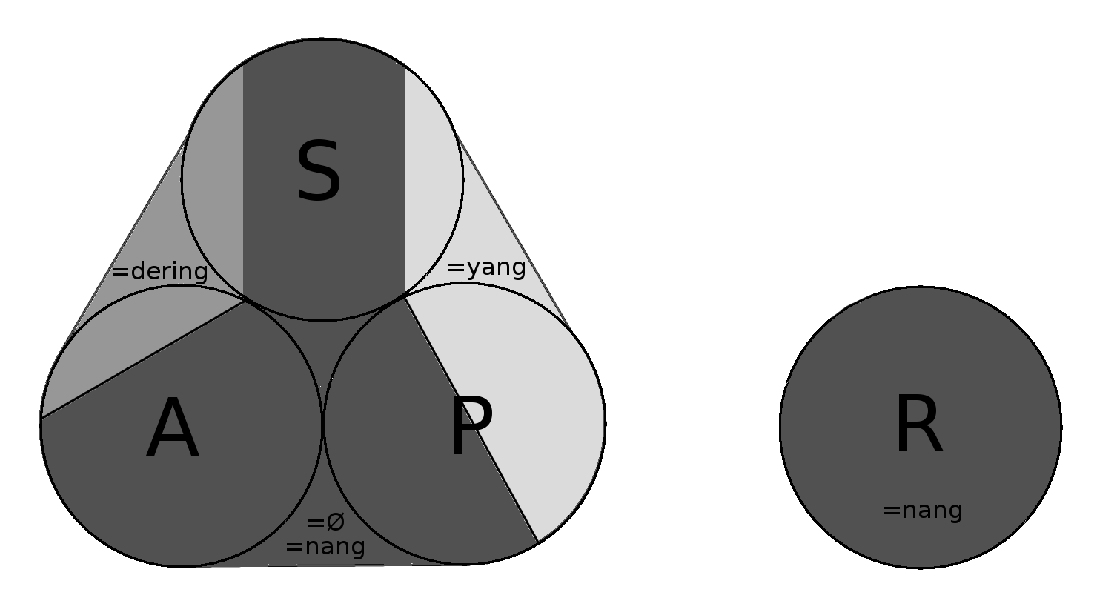
\includegraphics[height=.3\textheight]{pics/sap-slm.eps}
 % argstr.eps: 1179666x1179666 pixel, 300dpi, 9987.84x9987.84 cm, bb=14 14 91 55
 \caption[Coding of semantic roles in SLM]{The coding of semantic roles in SLM. The instrumental \em =dering \em can code S and A, but is marginal, as seen by the small portion of the circles it covers. The accusative \em =yang \em can be used for P, where it is common, and for S, where it is marginal. This difference in frequency is represented by the different sizes of the covered surface. The dative marker \em =nang \em can be used for S, A and P, as can zero. For expository reasons, dative and zero are not distinguished in the illustration. Zero is much more frequent than the dative in all three roles. R finally can only be marked by the dative.}
 \label{fig:argstr}
\end{figure}


If we interpret this in terms of a theory of alignment, we find characteristics of accusative alignment and split-S alignment, as well as neutral alignment.

The role of the dative cannot be fit into any one of the standard types of alignment. Discussing these similarities in turn, we can say that the SLM system resembles accusative alignment if we discard the peripheral instances of institutional instrumentals and the rare cases of \em =yang \em attaching to S. In this case, S and A are always zero, while P is marked with \em =yang\em. We would  thus be dealing with a conflation of S and A, a nominative-accusative system. This ignores the dative marking for modals and experiencers, but this need not be a problem, since other languages with `dative subjects', like German for instance, are also commonly called nominative-accusative languages.

On the other hand, if we think that the institutional actors, and especially the instances of \em =yang \em found on S are indeed relevant, we find resemblances to a Split-S system. S is marked like A (zero or instrumental) if it is actor-like; if S is undergoer-like, it is marked like P (accusative).

When we turn to the most common case, the dative, we find resemblances to the neutral system in the sense that every argument \em can \em be marked with the dative. In a neutral system, there is no distinction between the arguments. However, in SLM, dative marking is normally not done simultaneously. It is rare that more than one argument is marked with the dative, so that it is possible to distinguish the semantic roles of the arguments, which is not what we find in a neutral system.

To sum up, the SLM system shows resemblances to a number of alignment systems, but is not a clear instance of any of them. This might have to do with the fact that the traditional alignment systems only take into account a mapping of  three roles on two cases (the tripartite system being somehow only of theoretical relevance). In SLM, we have more than two markings which are relevant, accusative, dative, zero and possibly the instrumental. These do not fit nicely in the classical S-A-P triangle (cf. Figure \ref{fig:argstr}), but rather cut across all of S, A and P. It appears that the three-circles model is thus not very appropriate for SLM. Rather, SLM seems to have a special kind of \em semantic alignment\em, which goes beyond the classical active-stative-split \citep{Klimov1974}.

One interesting thing to note about the dative is that it normally occurs in contexts with low volitionality (experiencer, modality, recipient). There might be a possibility to interpret the accusative as [+affected], the instrumental as [+active] and the dative as [-volitional] \citep{Ansaldo2005ms}. Arguments are marked for this if disambiguation requires it, otherwise, zero can be used. Crucially, the number of arguments of a predicate does not seem to influence the choice of a marker. The syntactic relevance of valency of predicates is thus limited, and it can indeed be argued that in SLM, predicates do not subcategorize for the number of arguments they take. The speaker is free to add as many referents to the predicate as he sees fit, and to suppress as many referents as he thinks will not impede understanding. Any referent can be dropped \formref{sec:grel:Pro-drop}, and the semantic role of any referent can be indicated by appropriate postpositions. In that sense, the four referents in \xref{ex:argstr:conclusion} are all of the same status, there is not one which would enjoy a privileged status over another in the way in which arguments are privileged over adjuncts.


\yboy{1}{
\ea \label{ex:argstr:conclusion}
\gll itthu    baathu=yang    incayang Seelong=dering laayeng nigiri=nang asà-baapi. \\
 \textsc{dist} stone=\textsc{acc} \textsc{3s.polite} Ceylon-\textsc{abl} other country=\textsc{dat} \textsc{cp}-bring\\
\z
}


% \yboy{1}{
% \ea
% \gll {\em police} dering seyang ana preksa. \\
%        \\
%     `.' (nosource)
% \z
% } \\
% 
% 
% \yboy{1}{
% \ea
% \gll {\em police} dering seeyang {\em remand} nang su kiiring. \\
%        \\
%     `.' (nosource)
% \z
% } \\
% 
% \yboy{1}{
% \ea
% \gll {\em police} dering su dhaathang. \\
%        \\
%     `.' (nosource)
% \z
% } \\

 
